O diâmetro do cabo é dado pela equação:
\begin{equation}
  d_c = Q\sqrt{T}
  \label{eq:diametro_do_cabo}
\end{equation}
Onde:
\begin{itemize}[leftmargin=1.25cm]
  \item $d_c$: diâmetro do cabo em $\si{\milli\meter}$.
  \item $Q$: coeficiente segundo a norma NBR 8400.
  \item $T$: força de tração no cabo em $\si{\deca\newton}$.
\end{itemize}
\vspace{1em}

O coeficiente Q foi obtido na tabela 27 da NBR 840:

\begin{figure}[H]
  \centering
  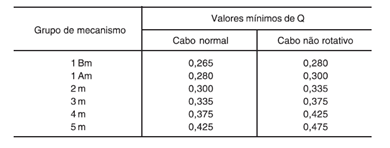
\includegraphics[width=0.5\textwidth]{content/sections/03_sistema_de_elevacao/images/04_coeficiente_q.png}
  \caption{Valores Mínimos de Q}
  \label{fig:coeficiente_q}
\end{figure}
\vspace{1em}

Para o grupo do mecanismo 1AM, o valor de Q para cabo normal é de $0,28$.
\vspace{1em}

Substituindo os valores na equação \eqref{eq:diametro_do_cabo}:
\begin{align*}
  d_c & = 0,28 \sqrt{2537,78}              \\
  d_c & = \boxed{\SI{14,11}{\milli\meter}}
\end{align*}
